\chapter{Test}

\section{Unit test}
Her testes, om terningerne følger den givne stokastiske variabel.

Her testes, om der er lige stor sandsynlighed for at vinde, når man er spiller 1 og spiller 2.

\section{Coverage test}
Coverage test (\textit{dansk: kodedækningstekst}) omhandler metoderne i ens program.
Testen går såmænd ud på, at spillet bliver kørt, og den registrerer, hvorvidt alle metoderne bliver brugt, eller om der er såkaldt død kode, der ikke bliver brugt i nogle sammehænge.
Code coverage måles i en procentsats, og det betragtes ud fra normale omstændigheder som acceptabelt, at programmets code coverage er på 70-80\% \footnote{Cornett, Steve; Minimum Acceptable Code Coverage, http://www.bullseye.com/minimum.html, last updated: 2013. }.
Årsagen til den tilsynelagende lave acceptable code coverage skyldes, at det kan være for tidskrævende at få en højere procentsats.
I sikkerhedssystemer vil man dog normalt bestræbe sig efter 100\% code coverage.
\\
Vi har brugt IntelliJs integreret code coverage-test, som ligesom Eclipses code coverage-plugin viser, efter endt program, de forskellige procentsatser på de forskellige klasser. En enkel kørsel af spillet viser nedenstående resultat (kun spillet er testet, ikke GUI'en, som har en masse metoder, som ikke bliver benyttet):
\begin{figure}
    \begin{center}
        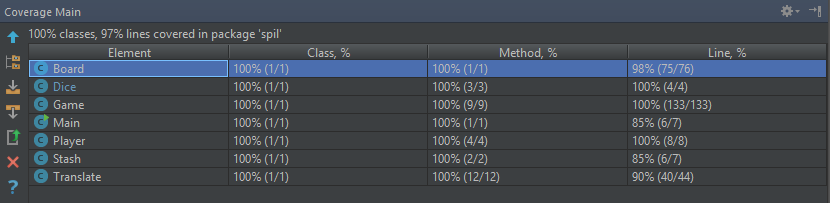
\includegraphics[width=15cm]{graphics/coveragetest/coveragetest1.png}
        \caption{Screen dump af code coverage}
        \label{fig:codecoverage}
    \end{center}
\end{figure}
\\ \\
Det fremgår af skærmbilledet, at alle procentsatser er >80\%, som der i større applikationer antages som acceptabelt. Ved at se, hvorfor nogle metoder ikke bliver brugt, så kan man ved at dykke ind i klasserne se, at eksempelvis bliver main-metoden i Main-klassen ikke bliver brugt. Ligeledes bliver der i Stash-klassen ikke brugt hele \textit{addAmount}-metoden, som det fremgår af skærmbilledet nedenunder:
\begin{figure}
    \begin{center}
        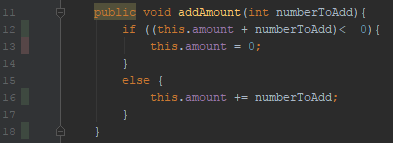
\includegraphics[width=8cm]{graphics/coveragetest/coveragetest2.png}
        \caption{Screen dump af addAmount}
        \label{fig:codecoverage_addamount}
    \end{center}
\end{figure}

\section{Testcases}
